\section{Motivation}
\label{sec:motivation}
\graphicspath{{_Intro/Figures/}}

\begin{figure}[!b]
	\centering
		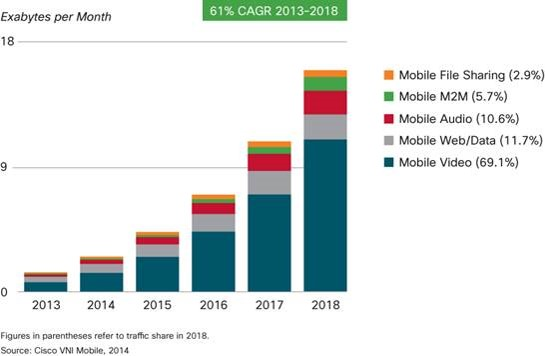
\includegraphics[width=3in]{vnigraph.jpg}
	\caption{Cisco VNI Forecast}
	\label{fig:vnigraph}
\end{figure}

The demand for wireless capacity to access the Internet has greatly increased with rise in use of mobile computing devices including, laptops, tablets, and phones. We are increasingly using the Internet to access articles, financial services, social networking, shopping, multimedia applications, gaming etc to name a few. There is ongoing research and increasing commercial activity in the field of smart spaces where everything from appliances, gadgets, power grid to home security are networked via cloud based services. The Cisco VNI forecast illustrated in \figurename{ \ref{fig:vnigraph}} predicts this potential increase in networked traffic from current estimates of 54 EB to nearly double to 107 EB by 2016,

With increase in use of mobile devices to access online services, wireless is increasingly the preferred method for internet access. This is currently being accomplished using the electromagnetic radiation within the RF spectrum. The RF bandwidth is a limited resource and the existing spectral allocations limit the ability to increase its capacity thus making it ever so difficult to keep up with the wireless demand. In contrast to RF, light-based communication, and particularly the visible spectrum, is underutilized and has the potential to be exploited to provide extra capacity to meet the demand for wireless communications especially for indoor spaces. 

\begin{figure}[!t]
	\centering
		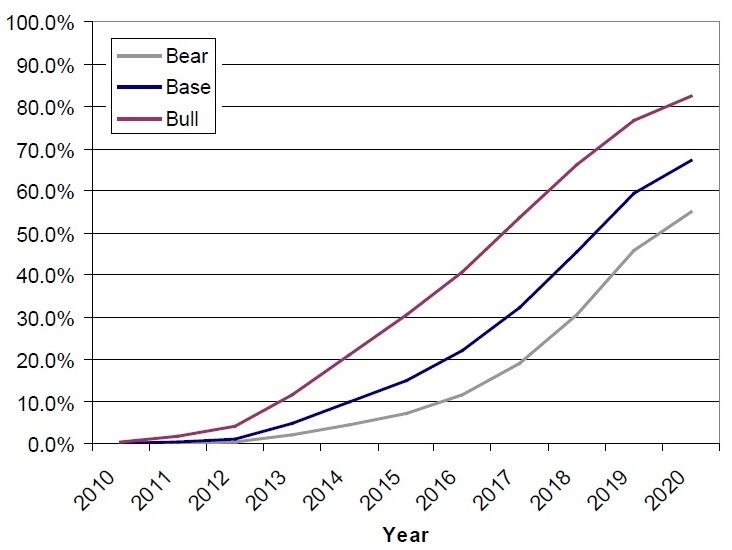
\includegraphics[width=4in]{socketpenetration.jpg}
	\caption{Total Cumulative Worldwide Socket Penetration}
	\label{fig:socketpenetration}
\end{figure}

Advances in solid state lighting has revolutionized the lighting industry. The realized energy and cost savings are leading the adoption of LEDs as the preferred source of illumination. \figurename{ \ref{fig:socketpenetration}} \cite{bar11a} predicts a worldwide socket penetration of atleast 55$\%$ by year 2020. The output luminous flux from an LED varies proportional to the current through the device. Information trasmission can be achieved by modulating the current at a relatively high frequency ($>~$200 Hz), generating a corresponding luminous flux, whose fluctuations are imperceptible to human eye. An optical receiver can sense this fluctuating illumination pattern and extract the transmitted information.

Under this model, each light in an indoor space can be deployed as a wireless access point while providing illumination. Directionality of light provides an extra layer of security. Deploying multiple devices within the indoor space enables spatial reuse over non-overlapping cones of illumination.
